\documentclass[a4paper,11pt]{article}

\usepackage[T1]{fontenc}
\usepackage[utf8]{inputenc}
\usepackage{graphicx}
\usepackage{xcolor}
\usepackage{calc}
\renewcommand\familydefault{\sfdefault}
\usepackage{tgheros}
\usepackage[defaultmono]{droidmono}
\usepackage{ amssymb }
\usepackage{amsmath,amssymb,amsthm,textcomp}
\usepackage{enumerate}
\usepackage{multicol}
\usepackage{tikz}
\usepackage{courier}
\usepackage[nomessages]{fp}% http://ctan.org/pkg/fp
\usepackage{xstring}% http://ctan.org/pkg/xstring
\usepackage{xparse}% http://ctan.org/pkg/xparse
\usepackage{lastpage}
\usepackage{geometry}
\usepackage{hyperref}
\geometry{total={210mm,297mm},
left=25mm,right=25mm,%
bindingoffset=0mm, top=20mm,bottom=20mm}


\linespread{1.3}

\newcommand{\linia}{\rule{\linewidth}{0.5pt}}

% my own titles
\makeatletter
\renewcommand{\maketitle}{
\begin{center}
\vspace{2ex}
{\huge \textsc{\@title}}
\vspace{1ex}
\\
\linia\\
\@author \hfill \@date
\vspace{4ex}
\end{center}
}
\makeatother
%%%

% custom footers and headers
\usepackage{fancyhdr}
\pagestyle{fancy}
\lhead{}
\chead{}
\rhead{}
\lfoot{Documentation}
\cfoot{}
\rfoot{Page $\thepage$ of $\pageref{LastPage}$}
\renewcommand{\headrulewidth}{0pt}
\renewcommand{\footrulewidth}{0pt}
%

% code listing settings
\usepackage{listings}

\lstset{%
  language = Octave,
  backgroundcolor=\color{white},   
  basicstyle=\footnotesize\ttfamily,       
  breakatwhitespace=false,         
  breaklines=true,                 
  captionpos=b,                   
  commentstyle=\color{gray},    
  deletekeywords={...},           
  escapeinside={\%*}{*)},          
  extendedchars=true,              
  frame=single,                    
  keepspaces=true,                 
  keywordstyle=\color{orange},       
  morekeywords={*,...},            
  numbers=left,                    
  numbersep=5pt,                   
  numberstyle=\footnotesize\color{gray}, 
  rulecolor=\color{black},         
  rulesepcolor=\color{blue},
  showspaces=false,                
  showstringspaces=false,          
  showtabs=false,                  
  stepnumber=2,                    
  stringstyle=\color{orange},    
  tabsize=2,                       
  title=\lstname,
  emphstyle=\bfseries\color{blue}%  style for emph={} 
} 

%% language specific settings:
\lstdefinestyle{Arduino}{%
    language = Octave,
    keywords={void, int boolean},%                 define keywords
    morecomment=[l]{//},%             treat // as comments
    morecomment=[s]{/*}{*/},%         define /* ... */ comments
    emph={HIGH, OUTPUT, LOW}%        keywords to emphasize
}


\begin{document}

\title{Implementation of MLPs for XOR function with Single Hidden Layer}

\author{Lalit Singh}

\date{\today}

\maketitle
\NewDocumentCommand{\ca}{s m}{
  \FPeval{\result}{clip(#2)}
  \IfBooleanTF{#1}% Condition on starred/unstarred version
    {% starred version \ca*{...}
      \StrSubstitute{\result}{.}{,}
    }{% unstarred version \ca{...}
      \StrSubstitute{#2}{.}{,\!}[\temp]% '.' -> ','
      \StrSubstitute{\temp}{*}{\cdot}[\temp]% '*' -> '\cdot'
      $\temp=\StrSubstitute{\result}{.}{,\!}$
    }
}
\section{MLP Structure}
This implementation of MLP for XOR function has following structure. It contains single hidden layer with a variable number of nodes.  The input layer contains two input nodes which accepts input parameters and a single bias node. The output layer consists of single node which gives the estimation for XOR function. In the algorithm presented below, the calculations are shown for 3 nodes and a single bias node in hidden layer.
$$
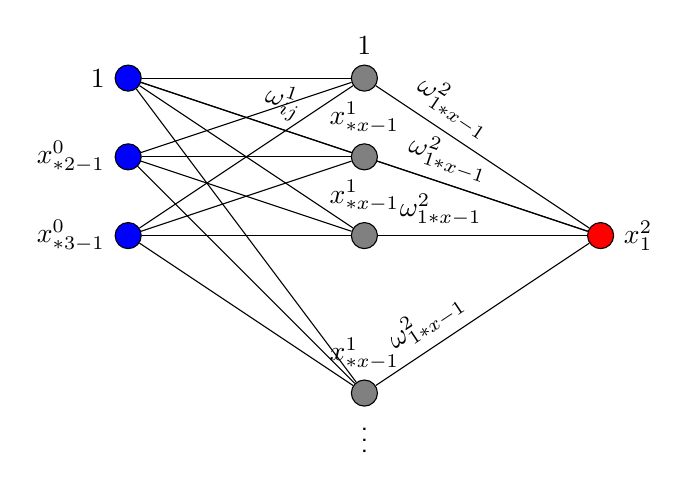
\begin{tikzpicture}
[   cnode/.style={draw=black,fill=#1,minimum width=3mm,circle},
]
    \node[cnode=red,label=0:$x_1^2$] (s) at (6,-3) {};
    % \node at (0,-4) {$\vdots$};
    \node at (3,-5.5) {$\vdots$};
	% \node at (6,-3.5) {$\vdots$};
    \foreach \x in {1,...,3}
    {
	% \ca*{2.5 + 2.78}
		\pgfmathparse{\x==1 ? 1 : "x_{\ca*{\x -1}}^0"}
        \node[cnode=blue,label=180:${\pgfmathresult}$] (x-\x) at (0,{-\x-div(\x,4)}) {};	
    }
	\draw (x-1) -- node[above,sloped,pos=0.3] {$\omega_{ij}^1$} (s);
	

    \foreach \x in {1,...,4}
    {   \pgfmathparse{\x==1 ? 1 : "x_{\ca*{x-1}}^1"}
        \node[cnode=gray,label=90:${\pgfmathresult}$] (p-\x) at (3,{-\x-div(\x,4)}) {};
    }
	
	
	\foreach \x in {1,...,4} {
		\pgfmathparse{\x==5 ? \x : "\omega_{1\ca*{x-1}}^2"}
		\draw (p-\x) -- node[above,sloped,pos=0.3] {${\pgfmathresult}$} (s);
	}
	
	
	
    \foreach \x in {1,...,3}
    {   \foreach \y in {1,...,4}
        {   \draw (x-\x) -- (p-\y);
        }
    }
\end{tikzpicture}
$$
\begin{figure}[h]
	\caption{Schema of MLP for XOR function with a single Hidden layer.}
\end{figure}
\section{Algorithm}
\large{\textbf{\underline{\textsc{Forward Pass:}}}}\\
The activation $x^1_{i = 1,2,...,n}$ of layer 1 is given by \\
\begin{equation} 
 x_i^m = \sigma
 \left(
 \sum_{j=1}^{L^{m-1}} w_{ij}^m x_j^{m-1} + w_{i0}^m
 \right)
\end{equation}
The above equation can be written in matrix form as below.\\
For Layer 1:
$$
\left[
\begin{matrix}
	x_1^1 \\ x_2^1 \\ x_3^1 \\\hdots
	\end{matrix}
\right]
=
\sigma
\left(
\left[
\begin{matrix}
	w_{10}^1 & w_{11}^1 & w_{12}^1\\
	w_{20 }^1& w_{21}^1 & w_{22}^1 \\
	w_{30}^1 & w_{31}^1 & w_{32}^1\\
	\hdots & \hdots & \hdots
\end{matrix}
\right]
\times
\left[
\begin{matrix}
	1\\ x_1^0 \\x_2^0\\
\end{matrix}
\right]
\right)
$$
\\
Similarly, for layer 2:
$$
\left[
\begin{matrix}
	x_{1}^2
\end{matrix}
\right]
=
\left[
\begin{matrix}
w_{10}^2 & w_{11}^2 & w_{12}^2 & w_{13}^2  & \vdots &
\end{matrix}
\right]
\left[
\begin{matrix}
1\\x_1^1\\x_2^1\\x_3^1 \\ \hdots \\  
\end{matrix}
\right]
$$
Note that, $\sigma$ is not applied for layer 2 because it is the ouput layer.
The number of nodes in the hidden layer can be extended to i = n by adding the weights $w^{1,2}_{i=4,...,n}$ and the activations $x^{1}_{3,...,n}$ in the space represented by $\vdots$ and $\hdots$ in above matrices.\\\\
The output of the \textbf{XOR} function is represented by the activation $x_1^2$ of node 1 of output layer.
\begin{equation}
	i.e. \hat{y} =\mathcal{N}_\theta(u) = x_1^2 
\end{equation}
\\
\large{\textbf{\underline{\textsc{Backward Pass:}}}}\\
Now, \\
The $\delta$ for $i^{th}$ node of layer m is defined as
\begin{equation}
\delta^m_i = \frac{\partial L(\mathcal{N}_\theta(u),y)}{\partial a_i^m}
\end{equation}
where L is the loss function and $a_i^m$ represents the potential of the $i^{th}$ node of layer m.\\\\
The \textsc{delta} for output layer is given by
\begin{equation}
	\delta_1^2 = 2(\hat{y} - y_i)
\end{equation}
And, the \textsc{delta} for the hidden layer can be computed by the formula given below:
\begin{equation}
\delta^m_i = \sigma'\left(a_i^m\right) \sum_{l = 1,...L^{m+1}} \delta_l^{m+1}w_{li}^{m+1}
\end{equation}
So the \textsc{delta} of hidden layer can be written in matrix form as given below:
$$
\left[
\begin{matrix}
\delta^1_0\\\delta^1_1\\\delta^1_2\\\delta^1_3
\end{matrix}
\right]
=
\sigma
\left(
\left[
\begin{matrix}
a_0^1 &  a^1_1 & a_2^1 & a_3^1
\end{matrix}
\right]
\right)
\times
\left[
\begin{matrix}
	w_{10}^2 &\vdots \\ w_{11}^2 &\vdots \\ w_{12}^2 &\vdots \\ w_{13}^2  & \vdots 
\end{matrix}
\right]
\times
\left[
\begin{matrix}
	\delta_1^2 \\\hdots
\end{matrix}
\right]
$$
The gradiant descent can be calculated is given by
\begin{equation}
	\frac{\partial L(\mathcal{N}_\theta(u),y)}{\partial w_{ij}^m} = \delta^m_i x_j^{m-1}
\end{equation}
\\
Also, in matrix form for layer 1:
$$
\left[
\begin{matrix}
	\dot{w}_{10}^1 & \dot{w}_{20}^1 & \dot{w}_{30}^1 & \vdots\\
	\dot{w}_{11}^1 & \dot{w}_{21}^1 & \dot{w}_{31}^1& \vdots\\
	\dot{w}_{12}^1 & \dot{w}_{22}^1 & \dot{w}_{32}^1 & \vdots\\
\end{matrix}
\right]
= 
\left[
\begin{matrix}
	1\\x_1^0 \\x_2^0
\end{matrix}
\right]
\times
\left[
\begin{matrix}
	\delta_1^1 & \delta_2^1 & \delta_3^1
\end{matrix}
\right]
$$
In matrix form for layer 2:
$$
\left[
\begin{matrix}
	\dot{w}_{10}^2 &\vdots \\ \dot{w}_{11}^2 &\vdots \\ \dot{w}_{12}^2 &\vdots \\ \dot{w}_{13}^2  & \vdots
\end{matrix}
\right]
= 
\left[
\begin{matrix}
		1\\x_1^1 \\ x_2^1 \\ x_3^1
\end{matrix}
\right]
\times
\left[
\begin{matrix}
\delta_1^2	
\end{matrix}
\right]
$$
% $$
% \left[
% \begin{matrix}
% 	\bar{\dot{w}}_{10}^1& \bar{\dot{w}}_{20}^1& \bar{\dot{w}}_{30}^1 & \vdots\\
% 	\bar{\dot{w}}_{11}^1 & \bar{\dot{w}}_{21}^1 & \bar{\dot{w}}_{31}^1 & \vdots\\
% 	\bar{\dot{w}}_{12}^1 & \bar{\dot{w}}_{22}^1 & \bar{\dot{w}}_{32}^1 & \vdots\\
% \end{matrix}
% \right]
% $$
Now the $\theta$ is updated by moving little bit in the direction of steepest decrease of the error:
\begin{equation}
\theta^{(n+1)} = \theta^{(n)} - \lambda\times \nabla R^{emp}(\mathcal{N})
\end{equation}
where $\lambda$ is learning rate. In this implimentation the value used for learning rate is 
$$\lambda = 0.1853 $$
In matrix form the weights can be updated as below:
$$
\left[
\begin{matrix}
	w_{10}^1 & w_{11}^1 & w_{12}^1\\
	w_{20 }^1& w_{21}^1 & w_{22}^1 \\
	w_{30}^1 & w_{31}^1 & w_{32}^1\\
	\hdots & \hdots & \hdots
\end{matrix}
\right]^{(n+1)}
=
\left[
\begin{matrix}
	w_{10}^1 & w_{11}^1 & w_{12}^1\\
	w_{20 }^1& w_{21}^1 & w_{22}^1 \\
	w_{30}^1 & w_{31}^1 & w_{32}^1\\
	\hdots & \hdots & \hdots
\end{matrix}
\right]^{(n)}
-
\lambda \times
\left(
\left[
\begin{matrix}
	w_{10}^1 & w_{11}^1 & w_{12}^1\\
	w_{20 }^1& w_{21}^1 & w_{22}^1 \\
	w_{30}^1 & w_{31}^1 & w_{32}^1\\
	\hdots & \hdots & \hdots
\end{matrix}
\right]^{(n)}
-
{
\left[
\begin{matrix}
	\bar{\dot{w}}_{10}^1& \bar{\dot{w}}_{20}^1& \bar{\dot{w}}_{30}^1 & \vdots\\
	\bar{\dot{w}}_{11}^1 & \bar{\dot{w}}_{21}^1 & \bar{\dot{w}}_{31}^1 & \vdots\\
	\bar{\dot{w}}_{12}^1 & \bar{\dot{w}}_{22}^1 & \bar{\dot{w}}_{32}^1 & \vdots\\
\end{matrix}
\right]^{(n)}}^\textbf{T}
\right)
$$

$$
\left[
\begin{matrix}
	w_{10}^2 &\vdots \\ w_{11}^2 &\vdots \\ w_{12}^2 &\vdots \\ w_{13}^2  & \vdots 
\end{matrix}
\right]^{(n+1)}
 = 
 \left[
 \begin{matrix}
 	w_{10}^2 &\vdots \\ w_{11}^2 &\vdots \\ w_{12}^2 &\vdots \\ w_{13}^2  & \vdots 
 \end{matrix}
 \right]^{(n)}
 -\lambda\times
 \left(
 \left[
 \begin{matrix}
 	w_{10}^2 &\vdots \\ w_{11}^2 &\vdots \\ w_{12}^2 &\vdots \\ w_{13}^2  & \vdots 
 \end{matrix}
 \right]^{{(n)}}
 -
 \left[
 \begin{matrix}
 	\dot{w}_{10}^2 &\vdots \\ \dot{w}_{11}^2 &\vdots \\ \dot{w}_{12}^2 &\vdots \\ \dot{w}_{13}^2  & \vdots
 \end{matrix}
 \right]^{(n)}
 \right)
$$

\section{Result}

The implementation of the algorithm is run by initializing the wights of the link with some random values. Initially the neural networks gives wrong output for most of input. With the increase in number of epoch the error in output decreases. After certain number of epoch ( \textit{the exact value depends upon randomly initialized weight values}), the error value start oscillating around certain value(\textit{again this values also depends upon the initial weights}). The algorithm is, then stopped, and the obtained weights are taken as optimal value for the given model.\newpage
The graph below shows the change in the error value of the with the increase in the number of epoch.
\begin{figure}[h]
\centering
\includegraphics[width=15cm]{Graph.png}
\caption{$\mathcal{N}_\theta(u)-y$ vs. number of epochs.The red colored stars represent  \textcolor{red}{error in output for input (0,0)} Similarly blue squares are for \textcolor{blue}{ error in output for input (1,0)}, greens are for \textcolor{green}{error in output for input (1,1)} and the cyan for \textcolor{cyan}{error in output for input (0,1)}}.
\end{figure}
\\The optimal weights value for the given model after 2000 epoches are given below:\\
$$
\left[
\begin{matrix}
	w_{10}^1 & w_{11}^1 & w_{12}^1\\
	w_{20 }^1& w_{21}^1 & w_{22}^1 \\
	w_{30}^1 & w_{31}^1 & w_{32}^1\\
\end{matrix}
\right]
=
\left[
\begin{matrix}
         0   &      0   &      0 \\
    0.0019  & -0.0015  & -0.0015 \\
         0   &      0   &      0 \\
	
\end{matrix}
\right]
$$
$$
\left[
\begin{matrix}
w_{10}^2 & w_{11}^2 & w_{12}^2 & w_{13}^2  &
\end{matrix}
\right]
=
10^{-3}
\left[
\begin{matrix}
	0.0000     &    0  & -0.4532  &       0\\
\end{matrix}
\right]
$$
\begin{thebibliography}{9}
\bibitem{knuthwebsite} 
Herbert Jaeger's Machine Learning Lecture Notes for Spring 2017
\\
\href{http://minds.jacobs-university.de/sites/default/files/uploads/teaching/lectureNotes/LN\_ML4IMS.pdf}{\texttt{http://minds.jacobs-university.de/sites/default/files/uploads
/teaching/lectureNotes/LN\_ML4IMS.pdf}}
\end{thebibliography}
\end{document}
